%%%%%%%%%%%%%%%%%%%%%%%%%%%%%%%%%%%%%%%%%
%
% (c) 2019 by Jennifer Laaser
%
% This work is licensed under the Creative Commons Attribution-NonCommercial-ShareAlike 4.0 International License. To view a copy of this license, visit http://creativecommons.org/licenses/by-nc-sa/4.0/ or send a letter to Creative Commons, PO Box 1866, Mountain View, CA 94042, USA.
%
% The current source for these materials is accessible on Github: https://github.com/jlaaser/pogil-polymers
%
%%%%%%%%%%%%%%%%%%%%%%%%%%%%%%%%%%%%%%%%%

\renewcommand{\figpath}{content/polymchem/freeradical/FRPchemistry/figs}
\renewcommand{\labelbase}{FRPchemistry}

\begin{activity}[Chemistry of Free-Radical Polymerization]

\begin{instructornotes}
	This activity introduces students to concepts related to the chemistry of free-radical polymerization.
	
	After completing this activity, students will be able to:
	\begin{enumerate}
		\item Draw appropriate mechanisms for the initiation, propagation, termination, and chain-transfer steps of a free radical polymerization
		\item Identify common initiators and the fragments that they leave on the ends of polymer chains
		\item Explain why free-radical polymerization typically results in head-to-tail addition of monomers
		\item Explain how different termination modes affect the end-group functionality and chain length of polymers produced by free radical polymerization
	\end{enumerate}
	
	\subsection*{Activity summary:}
	\begin{itemize}
		\item \textbf{Activity type:} Learning Cycle
		\item \textbf{Content goals:} Chemistry of free-radical polymerization
		\item \textbf{Process goals:} %https://pogil.org/uploads/attachments/cj54b5yts006cklx4hh758htf-process-skills-official-pogil-list-2015-original.pdf
			written communication, critical thinking, information processing
		\item \textbf{Duration:} TBD
		\item \textbf{Instructor preparation required:} none beyond knowledge of relevant content
		\item \textbf{Related textbook chapters:}
			\begin{itemize}
				\item \emph{Polymer Chemistry} (Hiemenz \& Lodge): section NNN
			\end{itemize}
		%\item \textbf{Facilitation notes:}
		%	\begin{itemize}
		%		\item \dots
		%	\end{itemize}
	\end{itemize}
	
\end{instructornotes}


\begin{model}[Initiation]
	\label{\labelbase:mdl:FRPinitchem}

	In a free-radical polymerization, the reactive species is a radical at the ``active'' end of each polymer chain.  Thus, the first step in a free radical polymerization is to generate an active radical species.  We refer to this step as \emph{initiation}.
	
	Shown below are two common chemistries used to generate initiator radicals in free-radical polymerizations:
	
	\begin{enumerate}
		\item Thermal decomposition of azobisisobutyronitrile (AIBN):
	
			\centerline{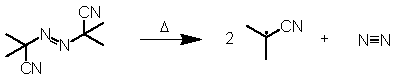
\includegraphics[scale=1.25]{\figpath/Model1-AIBN.pdf}}
			
		\item Thermal decomposition of benzoyl peroxide:
	
			\centerline{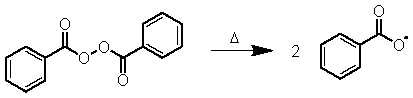
\includegraphics[scale=1.25]{\figpath/Model1-BPO.pdf}}
			
	\end{enumerate}
	
	%Note: this paper addresses the issue of benzoyl peroxide's further decomposition to phenyl radicals: 10.1021/ma00231a042 - it looks like it really is mostly the ester radical that adds about 95% of the time.
	
\end{model}


\begin{ctqs}

	\question On the left-hand side of each reaction, how many molecules are present?  Are any of them radicals?
	
		\begin{solution}[0.5in]
		\end{solution}
	
	\question On the right-hand side of each reaction, how many molecules are present? Are any of them radicals?
	
		\begin{solution}[0.5in]
		\end{solution}
	
	\question Briefly describe, in 1-2 complete sentences, why these reactions are useful for generating radical species in free radical polymerizations.
	
		\begin{solution}[1.5in]
		\end{solution}
		
	\question Ideally, the radical, which we often abbreviate \ce{I^.}, will go on to attack a monomer and start a polymer chain, as shown schematically below:
	
			\centerline{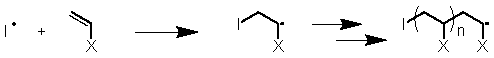
\includegraphics[scale=1.25]{\figpath/Model1-prop.pdf}}
	
		\begin{enumerate}
			\item Does the initiator radical become a permanent part of the polymer chain?  If so, where is it located?
	
				\begin{solution}[1in]
				\end{solution}
			
			 \item Shown below is the structure of a polymer produced by free-radical polymerization:
	
			\centerline{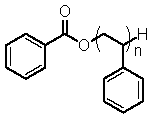
\includegraphics[scale=1.25]{\figpath/Model1-polymstruct.pdf}}
	
			What initiator was used in this polymerization?  In 1-2 complete sentences, briefly explain how you know.
	
				\begin{solution}[2in]
				\end{solution}
			
			\item If the same polymerization had been carried out using the other initiator shown in Model \ref{\labelbase:mdl:FRPinitchem}, what would the structure of the resulting polymer be?  Make sure to include the relevant end group(s).
	
				\begin{solution}[2in]
				\end{solution}
				
		\end{enumerate}
		
	\question Some initiator fragments may also undergo side reactions such as the recombination reaction shown below:
	
			\centerline{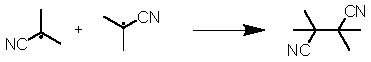
\includegraphics[scale=1.25]{\figpath/Model1-recomb.pdf}}
			
				How do you expect these types of side reactions to affect the overall ``efficiency'' of initiation in a free-radical polymerization? Briefly explain your reasoning in 1-2 complete sentences.
	
				\begin{solution}[1.5in]
				\end{solution}

\end{ctqs}



\begin{model}[Propagation]
\label{\labelbase:mdl:FRPpropchem}

	The second important step in a free radical polymerization is \emph{propagation}.  In this step, an active polymer chain radical attacks a monomer and links it to the chain, as shown below:
	
			\centerline{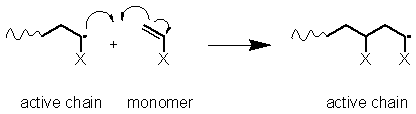
\includegraphics[scale=1.25]{\figpath/Model2-prop1.pdf}}
	
	For convenience, we will often abbreviate the active polymer chain as \ce{P^.}, in which case the propagation step can be depicted as:
	
			\centerline{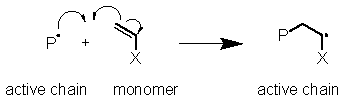
\includegraphics[scale=1.25]{\figpath/Model2-prop2.pdf}}
	

\end{model}

\begin{ctqs}

	\question Briefly describe what happens to the radical in the propagation step shown in Model \ref{\labelbase:mdl:FRPpropchem}.%Does the number of radicals present in the polymerization change during a polymerization step?  If so, how?
	
		\begin{solution}[1.5in]
		\end{solution}
	
	\question Does the length of the polymer chain change during a propagation step?  If so, how?
	
		\begin{solution}[1.25in]
		\end{solution}
	
	\question In Model \ref{\labelbase:mdl:FRPpropchem}, the radical is shown attacking the less-substituted side of the monomer (often called its ``tail'').  
	
		\begin{enumerate}
			\item This process is shown explicitly for polystyrene, below:
	
			\vspace{6pt}
			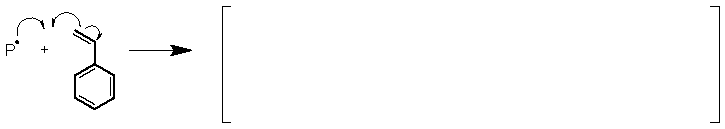
\includegraphics[width=\linewidth]{\figpath/Model2-styrene-tail.pdf}
			\vspace{6pt}
			
				Draw the product expected from this reaction in the space above, making sure to include any relevant resonance structures.
				
				\vspace{12pt}
			\item Alternatively, the radical could have attacked the more-substituted side of the monomer (the ``head''), as shown below:
			
			\vspace{6pt}
			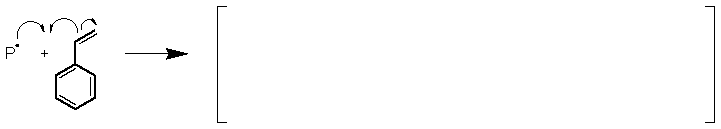
\includegraphics[width=\linewidth]{\figpath/Model2-styrene-head.pdf}
			\vspace{6pt}
			
				Draw the product expected from this reaction in the space above, making sure to include any relevant resonance structures.
				
				\vspace{12pt}
			\item Which version of this reaction produces the more favorable product, and why?
				
				\begin{solution}[1.5in]
				\end{solution}
			
			\item The different types of linkages that can be produced in a free-radical polymerization are summarized below (the linkage in question is shown with a dotted bond):
	
			\centerline{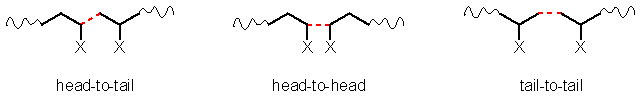
\includegraphics[scale=1.25]{\figpath/Model2-linkages.pdf}}
			
				Why does free-radical polymerization usually produce ``head-to-tail'' linkages?  Explain your team's reasoning in 2-3 complete sentences.
				
				\begin{solution}[2in]
				\end{solution}
			
		\end{enumerate}
		
	\question A propagation step using a different monomer, propylene, is shown below:
	
		\vspace{6pt}
			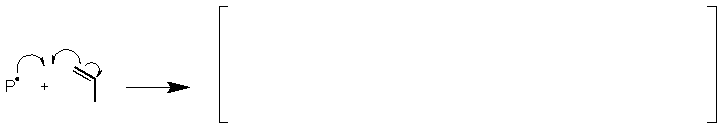
\includegraphics[width=\linewidth]{\figpath/Model2-propylene.pdf}
		\vspace{6pt}
	
		\begin{enumerate}
		
			\item Draw the product expected from this reaction in the space above, making sure to include any relevant resonance structures.
		\vspace{12pt}
			
			\item How do you expect the stability of the propagating radical in this reaction to compare to that generated from styrene?  Briefly explain your team's reasoning in 1-2 complete sentences.
			
				\begin{solution}[1.25in]
				\end{solution}
			
			\item Do you expect propylene to polymerize by free-radical polymerization?
			
				\begin{solution}[0.5in]
				\end{solution}
			
		\end{enumerate}
		
	\question Shown below are two groups of monomers:
	
			\centerline{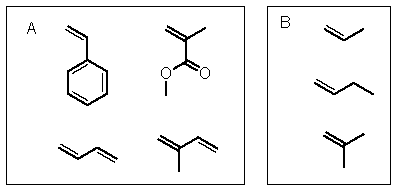
\includegraphics[scale=1.25]{\figpath/Model2-monomers.pdf}}
			
			Experimentally, it is found that the monomers in group A can be polymerized by free-radical polymerization, while those in group B cannot.
	
		In 3-4 complete sentences, explain the chemical origin of this finding, and briefly summarize the features necessary for a monomer to polymerize by free-radical polymerization.
			
				\begin{solution}[2.5in]
				\end{solution}

\end{ctqs}


\begin{model}[Termination]
\label{\labelbase:mdl:FRPtermchem}

	The final step in a free-radical polymerization is \emph{termination}, in which polymer radicals are deactivated to form chains that cannot polymerize further.
	
	The two important termination mechanisms in free-radical polymerization are termination by \emph{combination}:
	
			\centerline{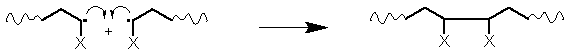
\includegraphics[scale=1.25]{\figpath/Model3-combination.pdf}}
	
	and termination by \emph{disproportionation}:
	
			\centerline{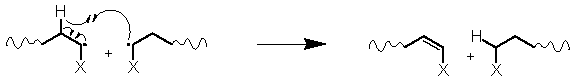
\includegraphics[scale=1.25]{\figpath/Model3-disprop.pdf}}

\end{model}

\begin{ctqs}

	\question How many polymer chains participate in each of the termination reactions shown in Model \ref{\labelbase:mdl:FRPtermchem}?
	
		\begin{solution}[0.5in]
		\end{solution}

	\question Why are the polymer chains on the right-hand side of each of these reactions considered to be ``dead'' chains that can no longer polymerize?
	
		\begin{solution}[1in]
		\end{solution}
	
	\question Two propagating polystyrene radicals are shown below:
	
			\centerline{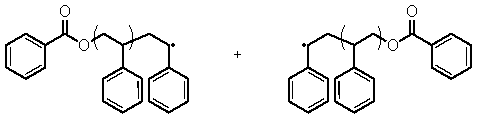
\includegraphics[scale=1]{\figpath/Model3-polystyrene.pdf}}
	
		\begin{enumerate}
			\item Draw the complete structure(s) of the product(s) formed if these radicals terminate by combination.
	
				\begin{solution}[1.5in]
				\end{solution}
			
			\item What type of linkage is formed in the middle of the resulting polymer chain?
	
				\begin{solution}[0.5in]
				\end{solution}
			
			\item How many initiator fragments does the resulting polymer chain contain?
	
				\begin{solution}[0.5in]
				\end{solution}
			
			\item How is the length of the resulting polymer chain related to the length of the propagating radicals that participated in the termination reaction?
	
				\begin{solution}[0.5in]
				\end{solution}
				
		\end{enumerate}
		
	\question For the same propagating polystyrene radicals discussed in the previous question,
	
		\begin{enumerate}
			\item Draw the complete structure(s) of the product(s) formed if these radicals terminate by disproportionation.
	
				\begin{solution}[1.5in]
				\end{solution}
			
			\item What type of functional group(s) are formed on the ends of the polymer chains?
	
				\begin{solution}[0.5in]
				\end{solution}
			
			\item How many initiator fragments does each of the resulting polymer chains contain?
	
				\begin{solution}[0.5in]
				\end{solution}
			
			\item How is the length of the resulting polymer chains related to the length of the propagating radicals that participated in the termination reaction?
	
				\begin{solution}[0.5in]
				\end{solution}
				
		\end{enumerate}
	
	\question In 3-4 complete sentences, briefly summarize the key differences between polymers that terminate by combination and those that terminate by disproportionation.
	
				\begin{solution}[3in]
				\end{solution}
	

\end{ctqs}

		

\begin{model}[Chain Transfer]
\label{\labelbase:mdl:FRPxferchem}

	A side reaction that can often occur during free radical polymerization is a ``transfer'' of the radical from the propagating chain to another molecular species, such as solvent.  This process is called \emph{chain transfer}.
	
	An example chain transfer reaction is shown below:
	
			\centerline{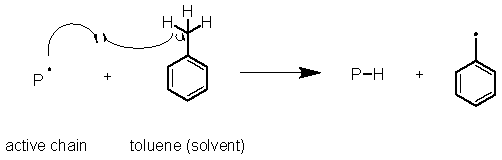
\includegraphics[scale=1.25]{\figpath/Model4-xfertoluene.pdf}}
	
\end{model}

\begin{ctqs}
	\question Explain, in 1-2 complete sentences, why we might say that chain transfer \emph{effectively} terminates the growing polymer chain:
	
		\begin{solution}[1.5in]
		\end{solution}
	
	\question Qualitatively, do you expect chain transfer to result in an increase, decrease, or no change in the molecular weight of the polymers produced in a free radical polymerization?
	
		\begin{solution}[1.5in]
		\end{solution}
		
\end{ctqs}


\begin{exercises}

	\exercise Indicate whether you expect each of the following factors to promote or inhibit formation of products in the reactions shown in Model \ref{\labelbase:mdl:FRPinitchem}, and briefly identify why: %Note: removed this one from Model 1, but I still like it
	
		\begin{enumerate}
			\item Energy required to break chemical bonds
	
				%\begin{solution}[0.75in]
				%\end{solution}
			
			\item Increase in the number of molecules present
	
				%\begin{solution}[0.75in]
				%\end{solution}
			
			\item Formation of a gaseous byproduct
	
				%\begin{solution}[0.75in]
				%\end{solution}
			
			\item Formation of resonance-stabilized products
	
				%\begin{solution}[0.75in]
				%\end{solution}
		\end{enumerate}
		
		Using your responses to the above questions, explain in 2-3 complete sentences why both of the initiators shown in \ref{\labelbase:mdl:FRPinitchem} decompose to form radicals when they are heated.
		
	
				%\begin{solution}[3in]
				%\end{solution}

	\exercise Draw the structure of a chain of poly(methyl methacrylate) prepared by free radical polymerization using AIBN as the initiator, assuming that all termination is by combination.  Make sure to show all relevant features of the polymer structure
	
	\exercise In Model \ref{\labelbase:mdl:FRPxferchem}, you considered chain transfer to solvent (toluene).  However, chain transfer can also take place between a radical chain and other molecular species in the reaction, which can have important consequences.
	
		\begin{enumerate}
			%\item Complete the following reaction scheme for chain-transfer to monomer:
			
			\item Complete the following reaction scheme for chain-transfer to polymer:
	
			\centerline{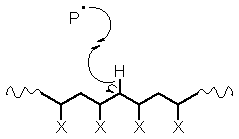
\includegraphics[scale=1.25]{\figpath/Model4-xferpolymer.pdf}}
			
			\item If the resulting radical species in part (b) then started adding additional monomers, what type of polymer architecture(s) could result?
		\end{enumerate}
	
\end{exercises}


%\begin{problems}
%
%	\problem First exercise
%	\problem Second exercise
%	
%\end{problems}


	
\end{activity}